\documentclass[11pt,a4paper]{article}

% Page layout
\usepackage[margin=2cm]{geometry}
\setlength{\parskip}{0.8em}
\setlength{\parindent}{0pt}

% Fonts and encoding
\usepackage[T1]{fontenc}
\usepackage[utf8]{inputenc}
\usepackage{lmodern}

% Math
\usepackage{amsmath, amssymb, amsfonts}

% Graphics
\usepackage{graphicx}
\usepackage{float}

% Colors and hyperlinks
\usepackage{xcolor}
\usepackage[hidelinks]{hyperref}

% Header and footer
\usepackage{fancyhdr}
\pagestyle{fancy}
\fancyhead[L]{}
\fancyhead[C]{}
\fancyhead[R]{}
\fancyfoot[C]{\thepage}

% Section formatting
\usepackage{titlesec}
\titleformat{\section}{\large\bfseries}{\thesection}{1em}{}
\titleformat{\subsection}{\normalsize\bfseries}{\thesubsection}{1em}{}

% Compact lists
\usepackage{enumitem}
\setlist{nosep}

\usepackage{natbib}

% For two-column layout if needed
% \usepackage{multicol}
% \setlength{\columnsep}{1cm}

% Title info
\title{Determine pinhole size}
\author{J.~M.~O. Massey}
\date{\today}
\begin{document}
\maketitle
\section{Introduction}

    \begin{figure}
        \centering
        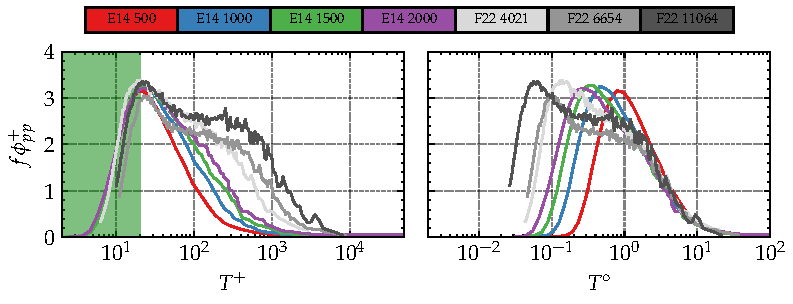
\includegraphics{figures/1_bl.pdf}
        \caption{Inner-scaled, pre-multiplied wall-pressure spectra in inner-(\textbf{left}) and outer-scaled (\textbf{right}) coordinates for a range of Reynolds numbers. The region $T^+\leq 20$ is highlighted in green. Data from \citet{eitel-amor_simulation_2014,fritsch_pressure_2020,fritsch_fluctuating_2022}}
    \label{fig:bl_spectra}
    \end{figure}

    In the measurement of wall pressure fluctuations in a turbulent boundary layer, we use a microphone cap with a pinhole (PH) to avoid spatial attenuation and aliasing effects. To reconstruct the measured pressure, we must calibrate the treated microphone setup and determine a transfer function ($H$) that maps $\mathrm{PH}\mapsto \mathrm{NKD}$, where NKD is the known pressure measurement. If the PH is too small, the suppression of the signal is too much and $H$ is ill-conditioned.

    Past data has shown that an inner- and outer-scaled part of the premultiplied wall-pressure spectra exist, with the inner-scaled part being invariant to frictional Reynolds number ($\delta^+\equiv \delta u_\tau / \nu$) \citep{massey_eddy_2025}. Figure \ref{fig:bl_spectra} shows that the peak of the inner-function sits at
    %
    \begin{equation}
        T^+\approx 20 ,
    \label{eq: temporal filter}
    \end{equation}
    %
    where the $\bullet^+$ superscript denotes normalisation by viscous units so that length scales $d^+\equiv d u_\tau/\nu$, time scales $t^+\equiv t u_\tau^2/\nu$, and frequency scales $f^+\equiv f \nu / u_\tau^2$. With this region of known behaviour, we can determine the size of the pinhole and correct accordingly.

\section{Spatial approximation using Taylor's frozen turbulence hypothesis}

    Convection velocity can be used to convert temporal fluctuations into spatial structures such that
    %
    \begin{equation}
        c_x^+ = \frac{\omega^+}{k_x^+} = (2\pi f^+) / (2\pi / \lambda_x^+) \;\;\Longrightarrow \;\; c_x^+ / \lambda_x^+ = f^+ .
    \end{equation}
    %
    Propagating the equality--acknowledging the relationship $T^+\equiv1/f^+$--established in \eqref{eq: temporal filter} leads to
    %
    \begin{equation}
        \frac{\lambda_x^+}{c_x^+} \lesssim 20,
    \end{equation}
    %
    where $c_x^+$ is the convection velocity and $\lambda_x^+$ is the wavelength of the structures. To minimise the attenuation of the smallest wavelengths, the pinhole diameter $d^+ = 0.5 {\lambda_x^+}_{\min}$ \citep{corcos_structure_1964}. The convection velocity of the pressure fluctuations is not constant throughout the boundary-layer \citep{willmarth_measurements_1962}, but a widely adopted approximation is $c_x^+\approx 10$ leading to
    %
    \begin{equation}
        \boxed{\frac{d u_\tau}{\nu} < 100.}
    \end{equation}

\section{Viscous scales in the Stanford wind tunnel}

    The plan is to deploy three pinholes, the largest is geared to the atmospheric conditions, the smallest to the highest $\delta^+$, maximum pressure, and one in between, the approximations are summarised in table~\ref{tab:stanford}.
    For this study, the boundary-layer thickness is assumed fixed at $\delta = 0.035~\mathrm{m}$ and the free-stream velocity is fixed at $U_{\mathrm{CL}} = 14~\mathrm{ms}^{-1}$.
    
    \begin{table}[H]
        \centering
        \begin{tabular}{c c c}
            $\sim \delta^+$ & $\nu/u_\tau$ [$\mu$m] & $d_{\max}$ [mm] \\
            \hline
            1500 & 23.33 & 2.33 \\
            5000 & 7.00 & 0.70 \\
            8200 & 4.27 & 0.43 \\
        \end{tabular}
    \label{tab:stanford}
    \end{table}



% \section{From measured pressure to a de-aliased wall-pressure spectrum}

% We denote by $\Phi_{xx}(f)$ the PSD of the raw microphone voltage and by $S(f)$ and $H_{\mathrm{PH}}(f)$
% the in-situ voltage--to--pressure calibration and the (calibrated) pinhole transfer, respectively.
% Let $\Phi_{nn}(f)$ be the facility-noise PSD (measured separately and/or removed using coherence).
% After calibration, pinhole deconvolution, and noise subtraction, the wall-pressure PSD estimate is
% \begin{equation}
% \widehat{\Phi}_{pp}(f)
% = \bigl|S(f)\,H_{\mathrm{PH}}(f)\bigr|^{-2}\,\Bigl[\Phi_{xx}(f)-\Phi_{nn}(f)\Bigr] .
% \label{eq:phicorr}
% \end{equation}

% \paragraph{Dimensional scalings.}
% Adopt the inner/outer variables used in \cite{massey_eddy_2025}:
% \[
% f^+ = \frac{f\,\nu}{u_\tau^2},\quad T^+=\frac{1}{f^+},\qquad
% T^\circ=\frac{U_e}{f\,\delta},\qquad
% \Phi_{pp}^+(f)=\frac{\Phi_{pp}(f)}{\tau_w^2},\ \ \tau_w=\rho u_\tau^2 .
% \]
% We will work with the premultiplied form $f\,\Phi_{pp}^+(f)$.

% \paragraph{Trusted band and model fit.}
% Define a trusted passband $B=[f_-,f_+]$ where the SNR is acceptable and
% $|S(f)H_{\mathrm{PH}}(f)|$ is well conditioned. Fit the two-population model
% from \cite{massey_eddy_2025} to the corrected spectrum on $B$ by minimising
% the premultiplied error:
% \begin{equation}
% \theta^\star
% =\arg\min_{\theta}\ \sum_{f_i\in B}
% \left[
% f_i\,\widehat{\Phi}_{pp}^+(f_i)
% - g_1\!\left(T_i^+;\theta\right)
% - g_2\!\left(T_i^\circ;\theta,\delta^+\right)
% \right]^2 ,
% \label{eq:fit}
% \end{equation}
% where $g_1,g_2$ are the inner/outer contributions (either Model~A: (3.1)–(3.2) or
% Model~B: (3.4), (3.9)–(3.10) in \cite{massey_eddy_2025}).

% \paragraph{Energy-consistent normalisation.}
% To lock the model amplitude to the data in $B$, scale the fitted model by
% \begin{equation}
% \alpha
% =\frac{\displaystyle\int_{B} \widehat{\Phi}_{pp}(f)\,d\ln f}
% {\displaystyle\int_{B} \Phi^{\mathrm{mdl}}_{pp}\!\left(f;\theta^\star,\delta^+\right)\,d\ln f},
% \qquad
% \Phi^{\mathrm{mdl}\star}_{pp}(f)=\alpha\,\Phi^{\mathrm{mdl}}_{pp}\!\left(f;\theta^\star,\delta^+\right).
% \label{eq:alpha}
% \end{equation}

% \paragraph{Model-based de-aliasing / spectral completion.}
% Outside $B$ the corrected measurement (\ref{eq:phicorr}) is attenuation/DAQ limited. Blend the
% measurement with the fitted model using a smooth taper $W(f)\in[0,1]$:
% \begin{equation}
% \Phi_{pp}^{\mathrm{DA}}(f)
% = W(f)\,\widehat{\Phi}_{pp}(f)
% + \bigl[1-W(f)\bigr]\ \Phi^{\mathrm{mdl}\star}_{pp}(f),
% \label{eq:blend}
% \end{equation}
% with, e.g., a cosine ramp of width $\Delta f$ on each side of $B$:
% \[
% W(f)=
% \begin{cases}
% 0, & f\le f_- - \Delta f,\\[2pt]
% \tfrac12\!\left[1+\cos\!\bigl(\pi \tfrac{f_- - f}{\Delta f}\bigr)\right], & f_- - \Delta f < f < f_-,\\[2pt]
% 1, & f_-\le f \le f_+,\\[2pt]
% \tfrac12\!\left[1+\cos\!\bigl(\pi \tfrac{f - f_+}{\Delta f}\bigr)\right], & f_+ < f < f_+ + \Delta f,\\[2pt]
% 0, & f\ge f_+ + \Delta f.
% \end{cases}
% \]
% Equation~\eqref{eq:blend} yields a de-aliased (completed) spectrum with the correct inner/outer
% asymptotics prescribed by the model.

% \paragraph{Outputs and checks.}
% The final premultiplied, de-aliased inner-scaled spectrum is
% \[
% f\,\Phi_{pp}^{+,\mathrm{DA}}(f)=\frac{f\,\Phi_{pp}^{\mathrm{DA}}(f)}{\tau_w^2}.
% \]
% Compute the variance and compare with known $\ln \delta^+$ trends:
% \begin{equation}
% \left\langle p_w'^2\right\rangle^+
% =\int_0^\infty f\,\Phi_{pp}^{+,\mathrm{DA}}(f)\,d\ln f,
% \qquad
% \text{cf. (\!3.14\!) channel and BL correlations in \cite{massey_eddy_2025}}.
% \label{eq:var}
% \end{equation}

% \paragraph{Notes.}
% (i) If desired, include DAQ anti-alias and sensor dynamics in $S(f)$ so that
% \eqref{eq:phicorr} uniformly corrects all linear filters. (ii) If the pinhole deconvolution
% is ill-conditioned for some $f$, shrink $B$ accordingly; the model will supply the spectrum
% there via \eqref{eq:blend}.





\bibliography{refs}
\bibliographystyle{jfm}

\end{document}